\begin{savequote}[75mm]
The beginning is the most important part of the work.
\qauthor{Plato, The Republic}
\end{savequote}

% pending plagiarism check
\begin{flushleft}
\chapter{Automated morphological profiling of patient derived organoids}

\section{A screening workflow for 3D organoid models}
To systematically measure morphological phenotypes of patient derived organoids and their morphological changes after treatment with a large number of compounds, I established a platform for high-throughput image-based drug profiling experiments (Figure 2a). Organoids were digested with a modified trypsin derivate, mechanically dissociated and filtered through a cell strainer to seed small fragments evenly onto 384-well imaging plates which were coated with a small volume of basement membrane extract. I standardized the amount and size of seeded organoid fragments in order to reliably measure organoid phenotypes after perturbation.
Also, the vertical distribution of organoid fragments within the BME layer was controlled in order to allow imaging of PDOs within the few captured confocal layers. In order to control the vertival distribution, I 
PDO fragments were incubated for three days to allow organoid formation before drug treatment. 
Subsequently, PDOs were treated with two compound libraries with a total of 527 small molecule inhibitors. Among them were 63 clinically used compounds that were added in 5 different concentrations (Clinical cancer library, N = 15 PDO lines) and a large experimental library (Ki-Stem library, N = 13 PDO lines) of 464 compounds (842 treatments in total; Figure S1 and Supplemental tables S3 and S4). 
Compounds were selected to target diverse developmental and signaling pathways, as well as clinically relevant targets for compound profiling. 
After four days of compound treatment, organoids were fixed and stained for actin (Phalloidin/TRITC), DNA (DAPI), and cell permeability (DeadGreen/FITC). Subsequently, plates were imaged at multiple z-positions by automated confocal microscopy. The procedure was repeated to generate two independent biological replicates of every PDO line.


\section{Selective 3D imaging of organoids during high-content imaging}
To rapidly analyze 3D imaging data of organoids, we developed a software framework called SCOPE (Selective 3D imaging for Contrast based Organoid Projection and feature Extraction). 
First, we projected the 3D image data onto a plane by applying a maximum contrast projection. 
This is an algorithm that uses the contrast surrounding a given pixel to determine the focal plane, allowing a precise structure detection and 2D representation of 3D objects. 
Next, individual organoids were segmented using a deep convolutional neural network. We developed a two-step procedure to establish segmentation: First, organoids were segmented based on fluorescence intensity of all channels. 
Then we used the intensity segmentation data to train a deep convolutional neural network for object identification. 
This improved the segmentation results by far, as observed by visual inspection (Figure 2b).
Subsequently, morphological profiles were calculated for each individual organoid, yielding 486 phenotypic features. 
These features include shape features, such as area and eccentricity, features describing the intensity distributions of each color channel, and texture features. 
Median and median absolute deviation of all features grouped on a well-wise level (973 features in total, including number of organoids per well as additional feature) showed a robust correlation between biological replicates (Figure 2d).


\section{Establishing patient derived organoids for high-throughput image-based profiling}

Patient derived organoids can be established from diverse healthy or malignant tissues and have been shown to represent their tissue and tumor of origin with respect to morphologic and molecular features including gene expression and mutations \cite{Fujii:2016jo, Weeber2015-sn, Van_De_Wetering2015-ko, Sato:2011-1h,  Broutier2017-wg}. To generate personalized cancer models for phenotypic compound screening, I built a standardized clinical and laboratory workflow to generate patient derived organoids from patients with colorectal cancer using endoscopic biopsy samples (Figure 1a). Briefly, fresh patient samples were washed and digested and rembedded in a basal membrane extract. The medium, termed ENA, was based on Advanced DMEM/F12 (Life technologies) and supplemented with growth factors, including Epidermal Growth Factor (EGF), the BMP-signaling antagonist Noggin and the small-molecule TGF\beta-signaling inhibitor A83-01. 

\begin{figure}[h]
\centering
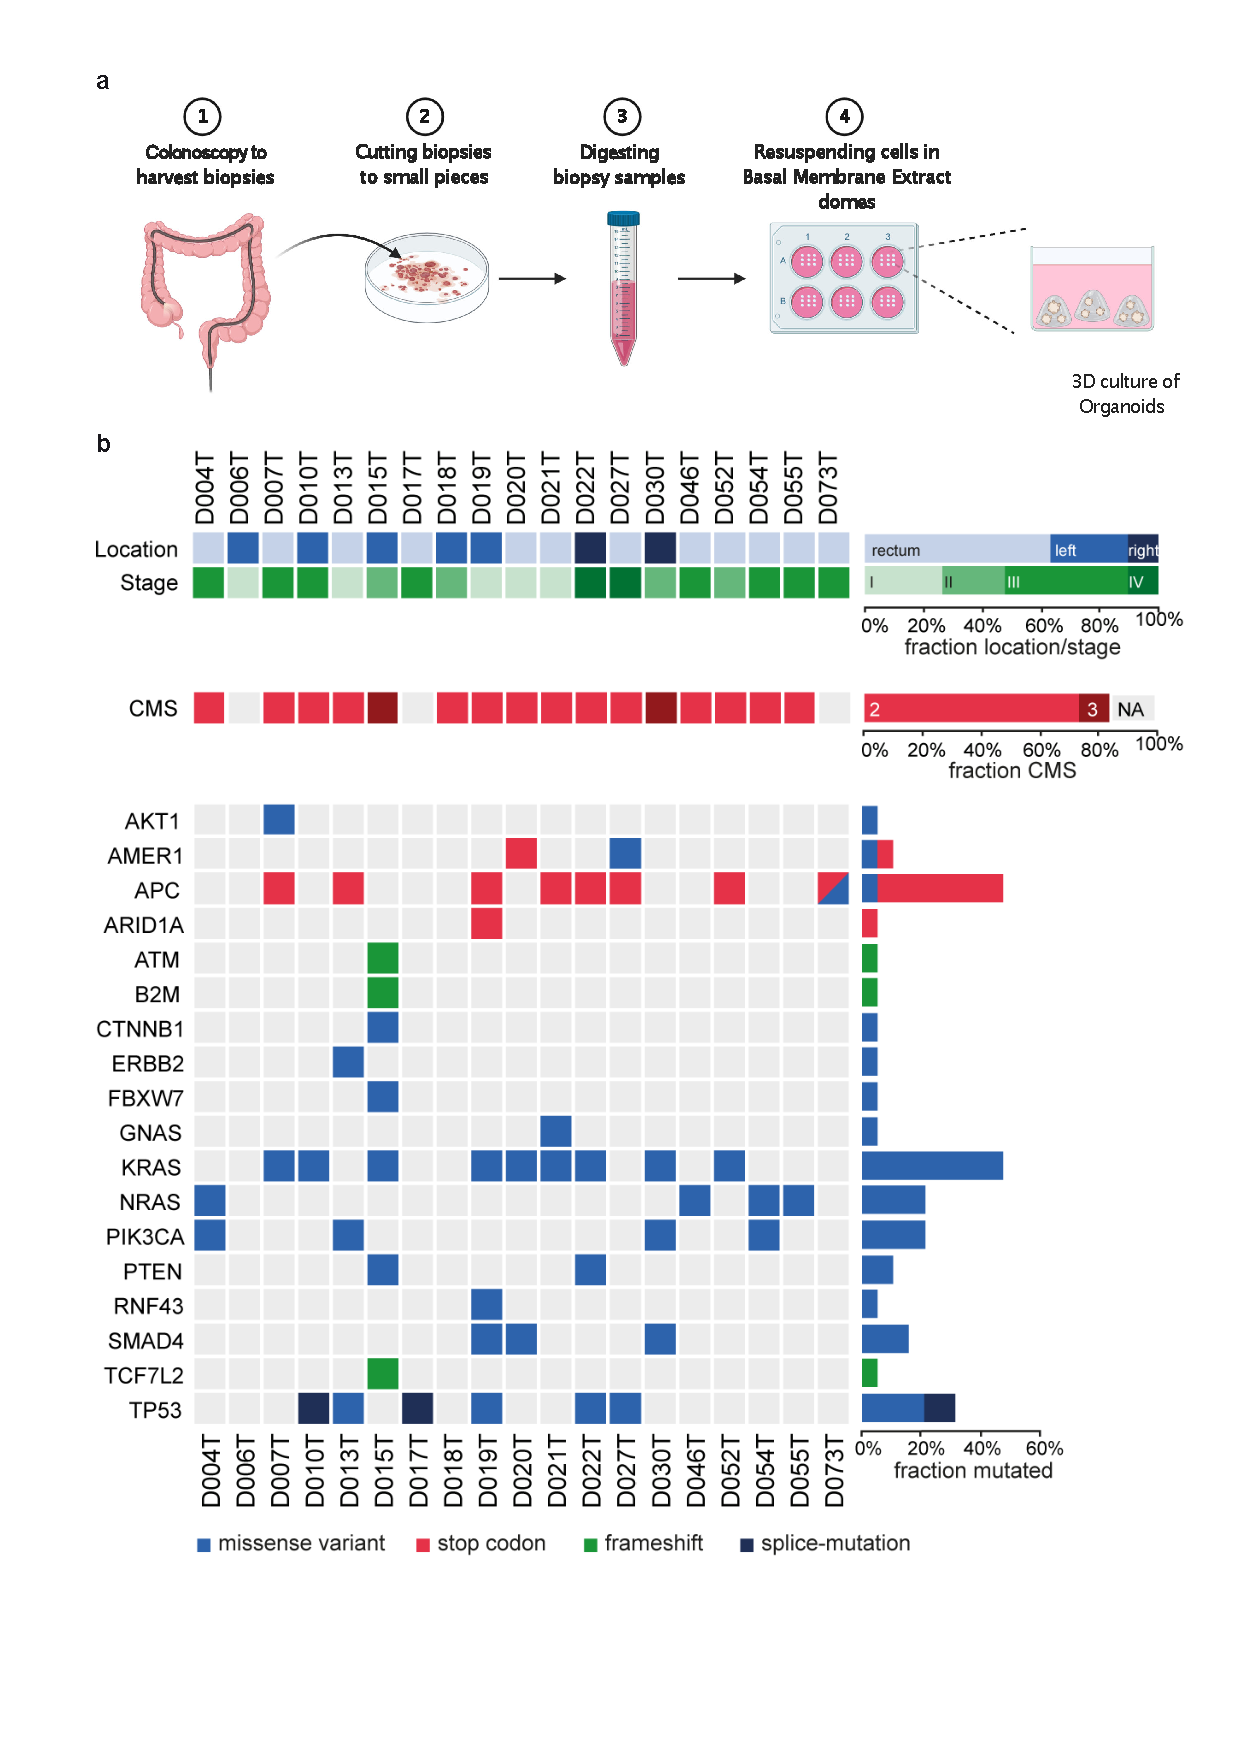
\includegraphics[width=\textwidth,
                height=\textheight,
                keepaspectratio]{figures/thesis_organoid_overview.pdf}
\caption{Organoid isolation and image-based profiling.}
\label{colon_cancer_progression}
\end{figure}

Patient derived organoids from 19 patients with colorectal cancer were prospectively developed. Donors to the biobank were representative of different UICC stages (Figure \ref{colon_cancer_progression}). Gene expression profiling and amplicon sequencing of frequently altered genes colorectal cancer showed molecular profiles characteristic for colorectal cancer (Figure 1c-d). Similar to sequencing studies of primary tumors, we observed a high frequency of APC (47\%), KRAS (47\%) and TP53 (36\%) mutations in patient derived organoid cultures \cite{Muzny2012-hr} (Figure 1d, Supplemental Table S2). On a gene expression level, patient derived organoids mainly represented the canonical consensus molecular subtype CMS 2 of colorectal cancer \cite{Guinney2015-ex}. No patient derived organoid line with a MSI-high phenotype and the associated CMS 1 molecular subtype was established. Also, no organoid line matched the molecular subtype CMS 4, which is associated with stromal infiltration and TGF\(\beta\)-signaling. These observations are in line with previous observations \cite{Van_De_Wetering2015-ko, Schutte2017-fl} and the limitations of the organoid culture system, which (1) selects for growth of intestinal epithelial cells and their progeny and (2) uses small molecule inhibitors of TGF\(\beta\)-signaling to ensure organoid proliferation \textit{ex vivo} \cite{Sato2011-lh}.

\end{flushleft}
